
\chapter{Results and Discussion}

The simulator capture sets of five perspective images and converts them into one image, mimicking the effect of fisheye lenses cameras. Using the setup described in Section~\ref{sec:combining_pictures}, and an calibratable polynomial lens model, each images is mapped onto specific parts of the final fisheye image. In Figure~\ref{fig:res_show_fisheye} the complete image is shown, simulating a $270^\circ$ FoV camera, mounted beneath the multirotor during flight. The simulator is fully implemented for Linux, but will work on Windows with some modifications to the build system and client program. This includes removing the ROS publisher, as ROS is currently not available on Windows platforms. No part of the simulator has been tested on Mac OS. 

\begin{figure}[!htb]
    \centering
    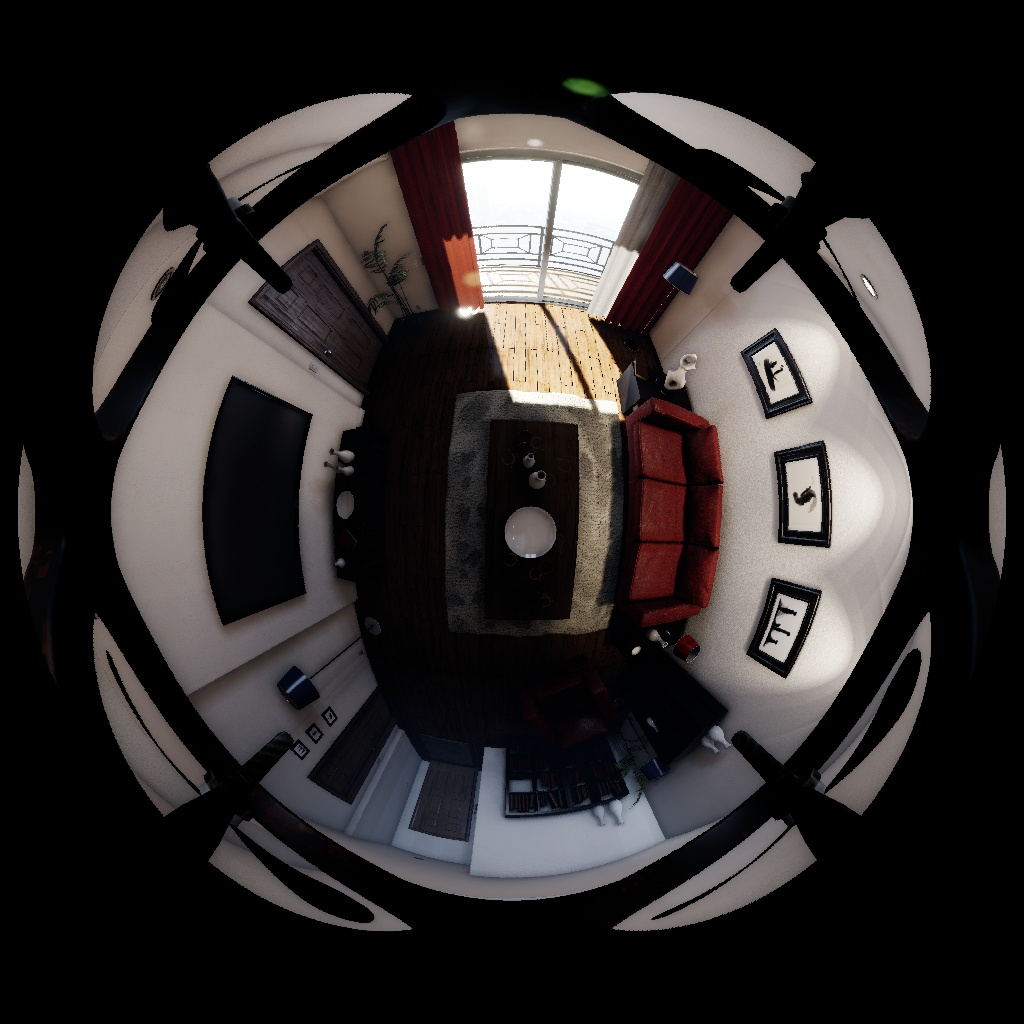
\includegraphics[width=0.7\textwidth]{rapport/fig/Results/1024to1024.jpeg}
    \caption{Simulated fisheye image taken in an indoor environment in Unreal Engine}
    \label{fig:res_show_fisheye}
\end{figure}

\section{Results}

The simulator is able to capture either single $90^\circ$ Fov pictures or full $270^\circ$ FoV pictures. This is because the simulator assumes the full five-camera setup, if it receives more than one image for transformation. The single pictures may be taken by any of the five cameras. This is donw by changing the image request sent to AirSim and setting the cameraposition as down, which tells the tranformer that the image does not need to be rotated.

The resolution settings for the perspective images can be set to a maximum of $4096\times4096$, and while there is no current limit to the resolution of the fisheye image, the height and width should should not exceed the double of the input image sizes. The FOV must equal $90^\circ$ for cube capture, but can be both increased and decreased for single captures, as long as the aspect ratio is preserved. 

\subsection{Fisheye captures and capture environment}

The images was taken in a indoor evironment provided by the Unreal Engine scene library. This is one of the freely available scenes in the Unreal Engine Library, and provides different types of lighting, some reflecting surfaces, as well as enough objects to be able to test the image quality. In Figure~\ref{fig:res_indoor_with_editor} the scene can be seen from editor view, while Figure~\ref{fig:res_original_pictures} shows five pictures taken from the multirotor inflight. All images shown in this comparison is taken with the default camera effect settings, which has a fast working auto exposure and no motion blur added. Picture noise is also tuned off.

\begin{figure}[!htb]
    \centering
    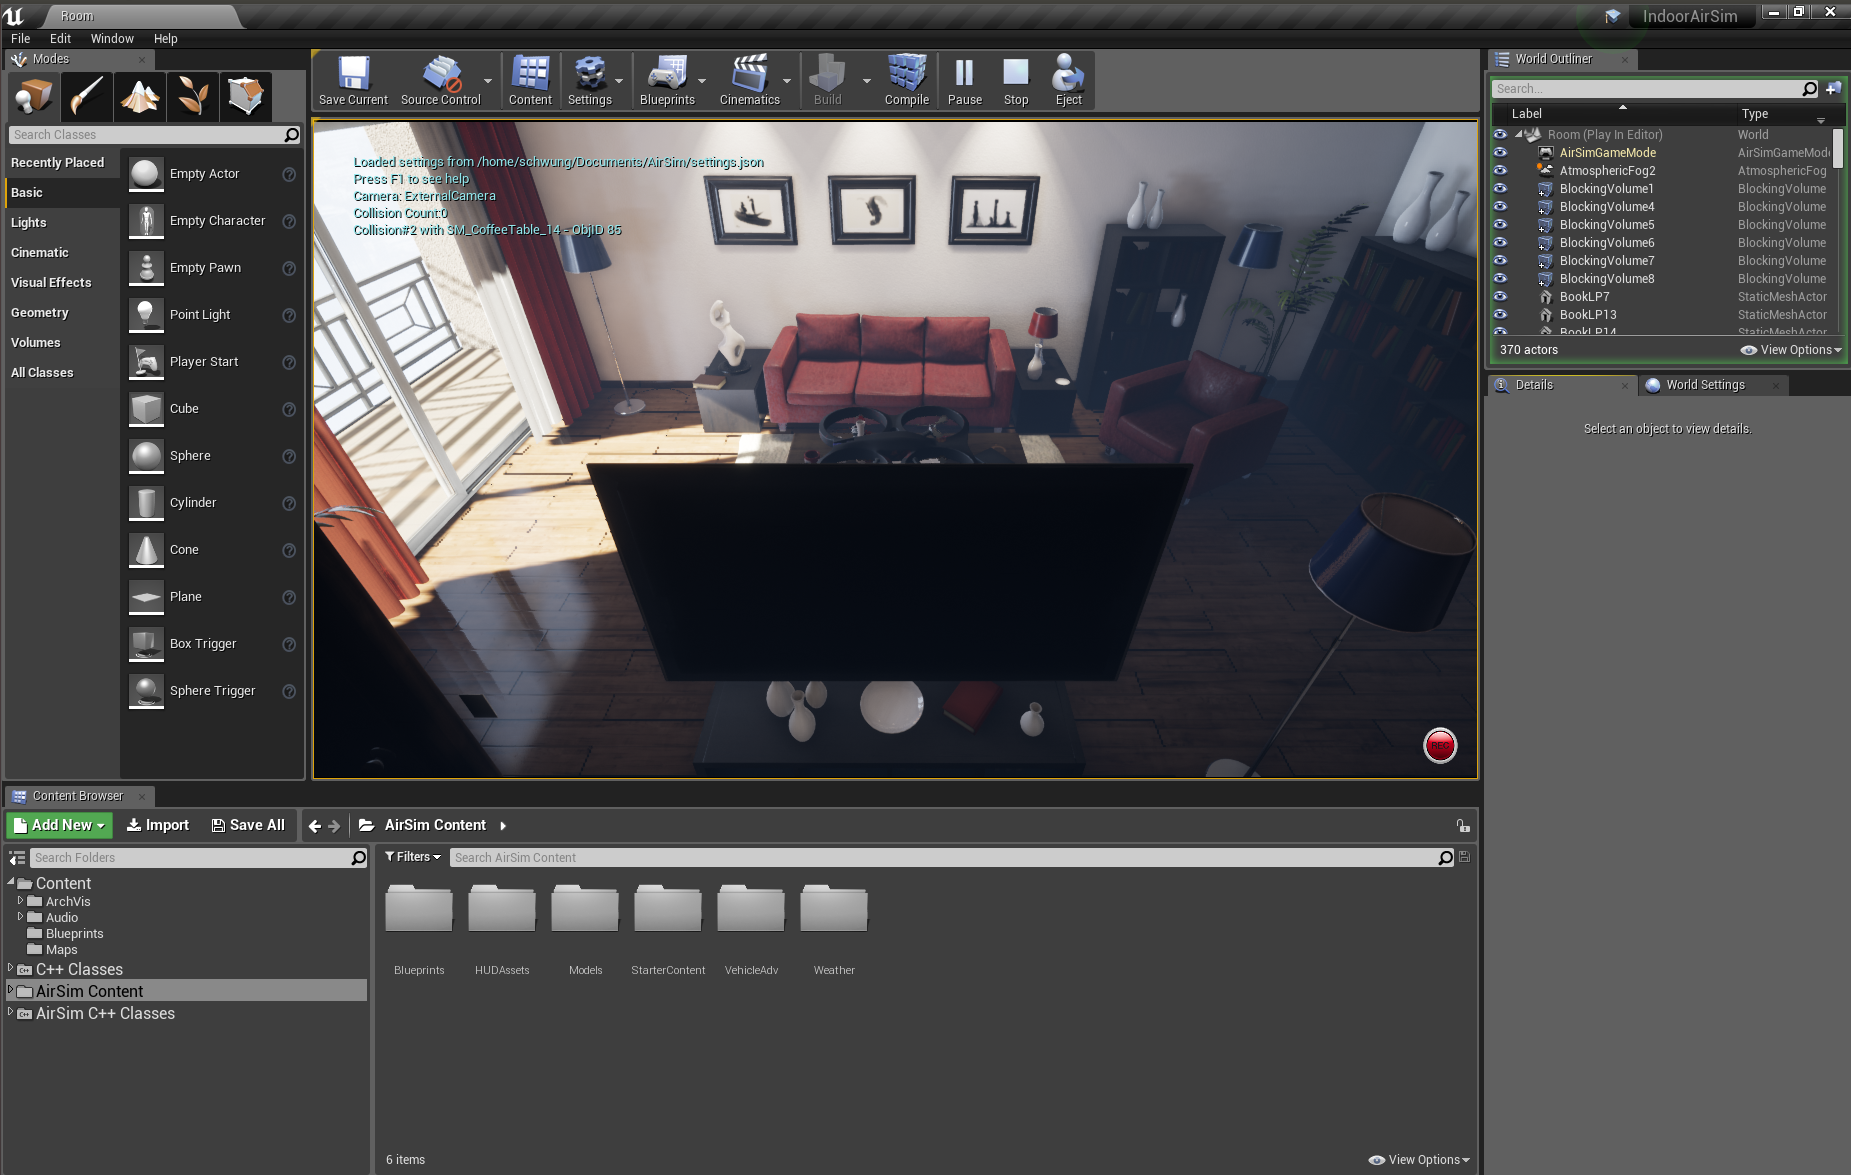
\includegraphics[width = 0.7\textwidth]{rapport/fig/Results/indoor_noconnect.png}
    \caption{Indoor test scene in the Unreal Engine editor}
    \label{fig:res_indoor_with_editor}
\end{figure}

The simulator will work in any environment created in Unreal Engine, by adding the project specific files along the AirSim files to the new scene. Figure \todo[inline]{add new environment} shows the same simulator in two other environments. The process of using pre-made scenes may be a bit tedious for Linux, since most scenes has been created for Windows. However, Unreal Engine provides tools for converting the projects to support Linux, and as of now all scenes have worked.

\begin{figure}[!htb]
    \centering
    \begin{subfigure}{0.32\textwidth}
    \centering
        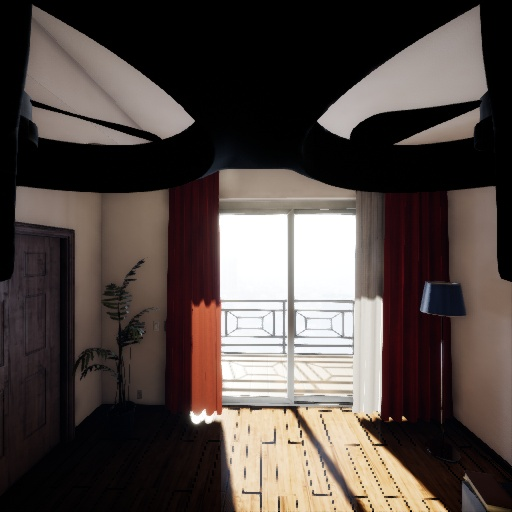
\includegraphics[height=5cm]{rapport/fig/Results/forward_center.jpeg}
        \caption{Front Camera}
        \label{fig:res_original_front}
    \end{subfigure}
    \begin{subfigure}{0.32\textwidth}
        \centering
        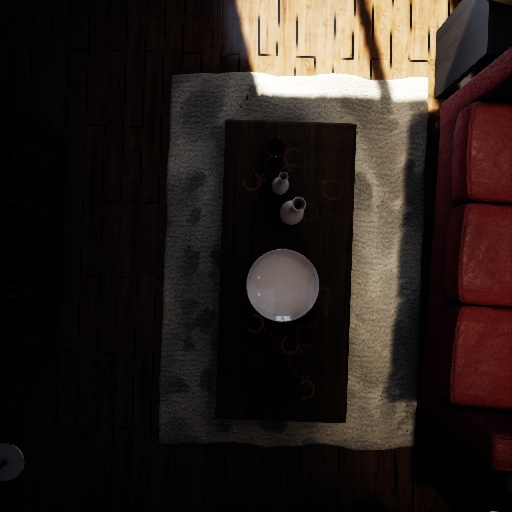
\includegraphics[height=5cm]{rapport/fig/Results/down_center.jpeg}
        \caption{Downward camera}
        \label{fig:res_original_down}
    \end{subfigure}    
    \begin{subfigure}{0.32\textwidth}
        \centering
        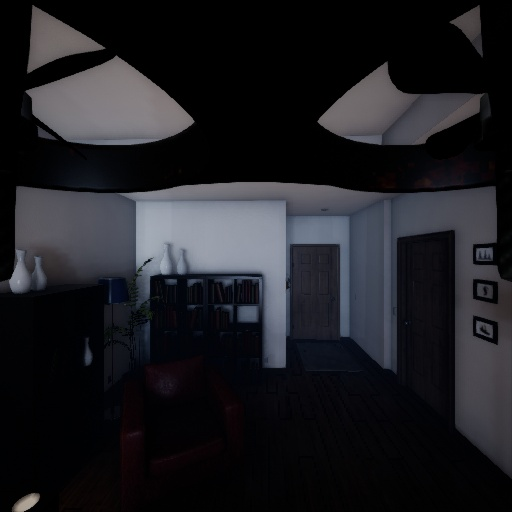
\includegraphics[height=5cm]{rapport/fig/Results/backward_center.jpeg}
        \caption{Back camera}
        \label{fig:res_original_back}
    \end{subfigure} \\[0.75ex]
    \begin{subfigure}{0.32\textwidth}
        \centering
        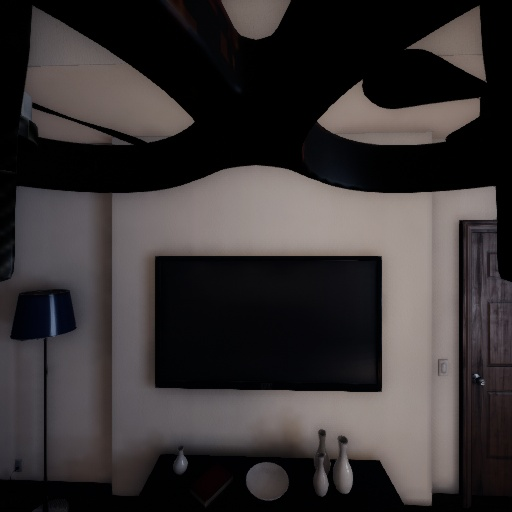
\includegraphics[height=5cm]{rapport/fig/Results/left_center.jpeg}
        \caption{Left Camera}
        \label{fig:res_original_left}
    \end{subfigure}
    \begin{subfigure}{0.32\textwidth}
        \centering
        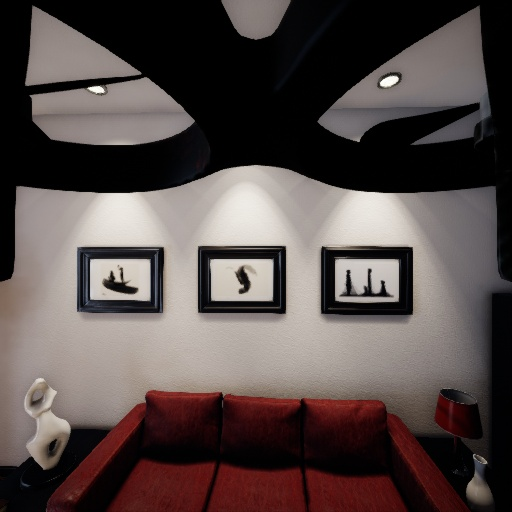
\includegraphics[height=5cm]{rapport/fig/Results/right_center.jpeg}
        \caption{Right Camera}
        \label{fig:res_original_right}
    \end{subfigure}
    \centering
    \caption{Comparison of image quality in different resolutions}
    \label{fig:res_original_pictures}
\end{figure}

In Figure~\ref{fig:res_quality_comparison} we see three images taken with different resolution, and using the lens parameters; $k_1 = 1.0$, $k_2=k_3=k_4=0$, creating an equiangular projection. The resolution in the compared pictures matches that of the perspective image resolution. This means that the $512\times512$ pixel image is combined from five $512\times512$ pixel images and so on. One can see that the image in Figure~\ref{fig:res_comp_256_to_256} is substantially lower than that of the image in Figure~\ref{fig:res_comp_1024_1024}. Almost all details on the door and railing are lost, and the reflection seen in the plate at the table is almost none existent. Comparing Figure~\ref{fig:res_comp_512_512} and Figure~\ref{fig:res_comp_1024_1024}, the differences are quite minimal.

\begin{figure}[!htb]
    \centering
    \begin{subfigure}{0.32\textwidth}
    \centering
        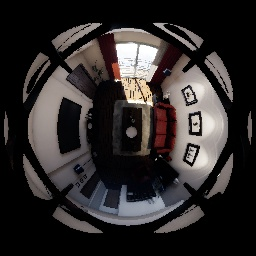
\includegraphics[height=5cm]{rapport/fig/Results/256to256.jpeg}
        \caption{$256 \times 256$ pixels}
        \label{fig:res_comp_256_to_256}
    \end{subfigure}
    \begin{subfigure}{0.32\textwidth}
        \centering
        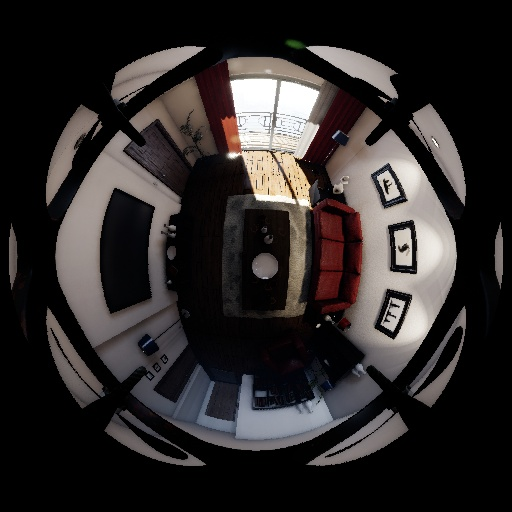
\includegraphics[height=5cm]{rapport/fig/Results/512to512.jpeg}
        \caption{$512 \times 512$ pixels}
        \label{fig:res_comp_512_512}
    \end{subfigure}    
    \begin{subfigure}{0.32\textwidth}
        \centering
        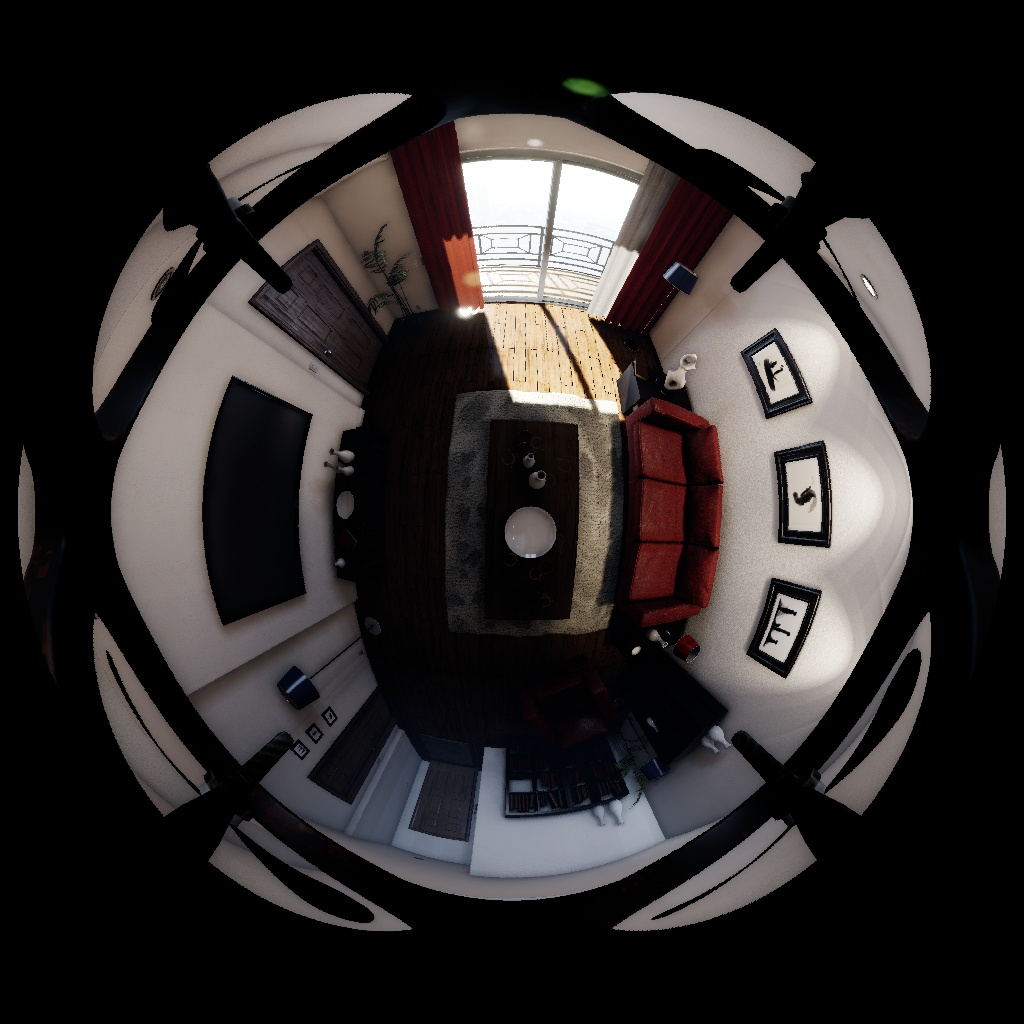
\includegraphics[height=5cm]{rapport/fig/Results/1024to1024.jpeg}
        \caption{$1024 \times 1024$ pixels}
        \label{fig:res_comp_1024_1024}
    \end{subfigure}
    \centering
    \caption{Comparison of image quality in different resolutions}
    \label{fig:res_quality_comparison}
\end{figure}

The images in Figure~\ref{fig:res_comp_equal} are taken with the same perspective image resolution of $512 \times 512$, but with two different destination resolutions. The most important difference here is the distortion lines seen in Figure~\ref{fig:res_comp_equal_512_1024}, caused by the stretching of the source image. However, it can also be seen that the detail level in the central parts have been increased.

\begin{figure}[!htb]
    \centering
    \begin{subfigure}{0.45\textwidth}
        \centering
        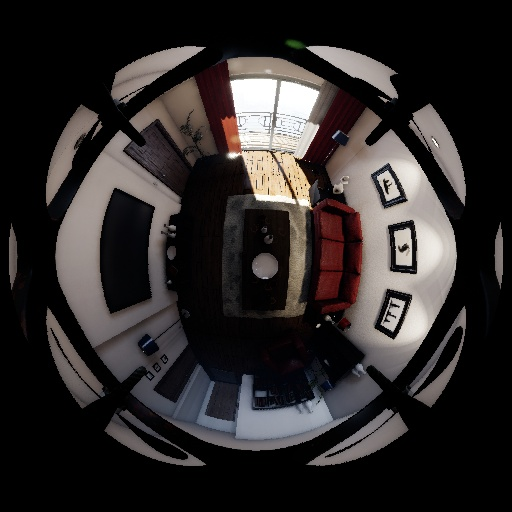
\includegraphics[height=7cm]{rapport/fig/Results/512to512.jpeg}
        \caption{$512 \times 512$ pixels}
        \label{fig:res_comp_equal_512_512}
    \end{subfigure}
    \begin{subfigure}{0.45\textwidth}
        \centering
        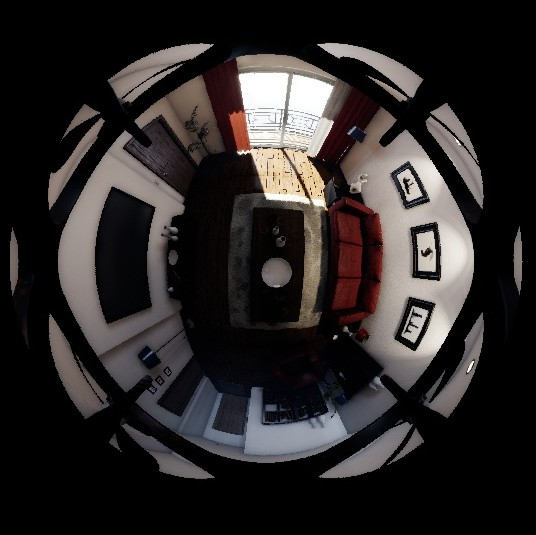
\includegraphics[height=7cm]{rapport/fig/Results/512to1024.jpeg}
        \caption{$1024 \times 1024$ pixels}
        \label{fig:res_comp_equal_512_1024}
    \end{subfigure}
    \caption{Comparison of transformed images with equal source resolution of $512 \times 512$}
    \label{fig:res_comp_equal}
\end{figure}

\subsection{Performance}

While the performance never was a part of the equation when implementing it, it is an important factor in a control application. All tests have been performed on the office PC in at NTNU. This PC does not have a dedicated graphics card, and Unreal Engine lagged considerably during tests. How much this affected the tests is unknown. however they should show qualitative data to shed some light upon areas to imporve the simulator.

Table~\ref{tab:res_timing_single} and \ref{tab:res_timing_cube_capture} show the timings in seconds for different resolutions and capture types. Note that while this is not even close to real time, all calculations done by the simulator are done sequentially for each pixel in the picture, meaning that no parallellization has been done. This can clearly be seen by comparing the calculation times, where the computation time follows the increase in resolution linearly. The fetch times are also higher for higher resolution picture, which are to be expected. Around $512\times 512$ it became quite noticable. 

\begin{table}[!htb]
    \centering
    \begin{tabular}{|c|c|c|c|} \hline
        \textbf{Input resolution} & \textbf{output resolution} & \textbf{Timing type} & \textbf{Time elapsed} \\ \hline \hline
        \multirow{2}{*}{$256 \times 256$} & \multirow{2}{*}{$512 \times 512$} & Fetch & 0.1 - 0.2 s \\ \cline{3-4}
         & & Transform & 0.4 s \\ \hline
        \multirow{2}{*}{$512 \times 512$} & \multirow{2}{*}{$512 \times 512$} & Fetch & 0.1 - 0.2 s\\ \cline{3-4}
         & & Transform & 1.5 s \\ \cline{2-4}
        \multirow{2}{*}{$1024 \times 1024$} & \multirow{2}{*}{$1024 \times 1024$} & Fetch &  0.3 - 0.5 s \\ \cline{3-4}
         & & Transform & 6.0 s \\ \hline
        \multirow{2}{*}{$2048 \time 2048$} & \multirow{2}{*}{$2048 \times 2048$} & Fetch & 0.6 - 0.7 s\\ \cline{3-4}
         & & Transform & 24.1 s\\ \hline
    \end{tabular}
    \caption{Timing for single capture transformation to fisheye image}
    \label{tab:res_timing_single}
\end{table}

\begin{table}[!htb]
    \centering
    \begin{tabular}{|c|c|c|c|} \hline
        \textbf{Input resolution} & \textbf{output resolution} & \textbf{Timing type} & \textbf{Time elapsed} \\ \hline \hline
        \multirow{2}{*}{$256 \times 256$} & \multirow{2}{*}{$256 \times 256$} & Fetch & 0.3 - 0.4 s\\ \cline{3-4}
         & & Transform & 2.0 s\\ \hline
        \multirow{4}{*}{$512 \times 512$} & \multirow{2}{*}{$512 \times 512$} & Fetch & 0.4 - 0.5 s \\ \cline{3-4}
         & & Transform & 7.9 s\\ \cline{2-4}
         & \multirow{2}{*}{$1024 \times 1024$} & Fetch & 0.4 - 0.5 s\\ \cline{3-4}
         & & Transform & 7.9 s\\ \hline
        \multirow{2}{*}{$1024 \time 1024$} & \multirow{2}{*}{$1024 \times 1024$} & Fetch & 0.7 s\\ \cline{3-4}
         & & Transform & 30.9 s\\ \hline
    \end{tabular}
    \caption{Timing for cube capture transformation to fisheye image}
    \label{tab:res_timing_cube_capture}
\end{table}


\section{Discussion}



\subsection{Image Quality}

\subsection{Performance and optimization}

\subsection{Task}

This project has not been a typical cybernetics project, and in many ways it shares more similarities with a computer science project. While the goal of was to extend the project to incorporate calibrating the fisheye camera to an actual camera, and possiby test computer vision algorithms on the platform, there hasn't been time. This is mainly because of lack of experience in critical areas. 

The project has had to handle very large code bases. Both the codebase of Unreal Engine and AirSim is quite extensive, as they both provide lots of functionality and features. While both platforms have a large user base, few of these discuss problems around the source code and the communication patterns within. Information regarding this is mostly limited to Github issues, and a few forum posts. While these problems became less relevant when making the client side application, it was a huge part of the development described in Section~\ref{sec:Early_dev}. 

Since the fisheye model was to be included into the AirSim interface, a deep understanding of the AirSim package was needed. Both in terms of internal dependencies, class and type definitions, coding style and communication patterns. The fact that it also had to incorporate new funtionality fom Unreal Engine meant that knowledge of C++ scripting towards Unreal Engine was needed. As the platform has an enormous amount of tools and funtionality available, there are also a lot of abstractions, to make the interface possible to use and develop for. However, the lack of previous experiece with game engines or Unreal Engine in particular, made this process quite time consuming. While reading through guides and watching tutorials

\subsection{Platform}

% This decision was made in order to separate the implementation into its own module, and thereby reducing the impact of changes to AirSim. As AirSim is still developed heavilly upon, it was seen as a way to reduce the amount trouble induced by changes to the core code of the plugin. This would also allow me to more often integrate the bug fixes and new implementations they made, without ruining my ownw work. The downside of this decision is that it removes possibility to use any features in Unreal Engine which is not implemented in the AirSim API. 


% \subsection{Project setup and programming environment}

% In this project I have forked both the EpicGames/Unreal Engine and the Microsoft/AirSim repository to my Github account, and made my own pivate repository for the project. This enable me to do specific changes to the source code of these projects, without the need to make pull requests to their original repositories. While AirSim is openly available, the source code of Unreal Engine is only available after being registered as a developer through their website. One requirement for getting the source code is that it is not distributed outside of this licencing. For this reason neither the fork of Unreal Engine, nor my own project repository are publicly available.

% Since one of the main goals of this project is the interfacing to ROS, the main OS for development will be Linux, specifically Ubuntu 18.04. However, since Unreal Engine is deeply integrated with Visual Studios, I will use Visual Studios on Windows as the main debugging platform, for everything except ROS. To build on Linux, I will use CMake, as they have done with AirSim. Both Unreal Engine and AirSim is built with the clang compiler, using libc++ as the standard library. However, the default ROS install uses libstdc++ as their standard library. This caused linking problems when combining ROS and AirSim. I therefore had to make some changes to the build and CMake scripts of AirSim in order to build with the GNU compiler g++, using libstdc++ as the standard library.

% \todo[inline]{Do I need to describe why this change is important?}

\cleardoublepage